\chapter{Notazione asintotica: le classi O, Omega, Theta grandi}

{{[}DFI{]} 2.2; {[}CLRS{]} 3.1}

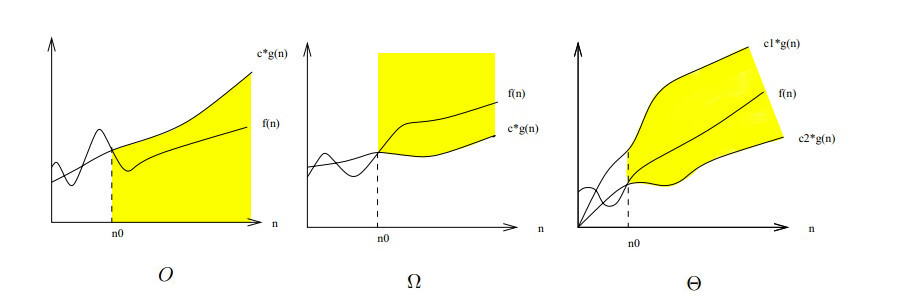
\includegraphics{images/classi_asintotiche.jpg}

Lettura della notazione: \\

$f(n) = \Theta(g(n))$ si legge: $f(n)$ è limitato strettamente da $g(n)$

\paragraph{Proprietà}

\subparagraph{Transitiva}

Se $f(n) = \Theta(g(n))$ e $g(n) = \Theta(h(n))$ allora $f(n) = \Theta(h(n))$ \\
Se $f(n) = O(g(n))$ e $g(n) = O(h(n))$ allora $f(n) = O(h(n))$ \\
Se $f(n) = \Omega(g(n))$ e $g(n) = \Omega(h(n))$ allora $f(n) = \Omega(h(n))$ \\
\\
Se $f(n) = o(g(n))$ e $g(n) = o(h(n))$ allora $f(n) = o(h(n))$ \\
Se $f(n) = \omega(g(n))$ e $g(n) = \omega(h(n))$ allora $f(n) = \omega(h(n))$


\subparagraph{Riflessiva}

$f(n) = \Theta(f(n))$ \\
$f(n) = O(f(n))$ \\
$f(n) = \Omega(f(n))$

\subparagraph{Simmetrica}

$f(n) = \Theta(g(n))$ se e solo se $g(n) = \Theta(f(n))$

\section{Limite superiore: Classe O grande}

O fornisce un limite superiore per la funzione $f(n), \forall n \geq n_0$

\begin{equation}
O(g(n)) = \{f(n) : \exists c,n_0 > 0 \in \mathbb{N}, 0 \leq f(n) \leq c*g(n), \forall n \geq n_0 \}
\end{equation}

\subsection{Limite inferiore: Classe Omega grande}

\Omega\, fornisce un limite inferiore per la funzione $f(n), \forall n \geq n_0$

\begin{equation}
O(g(n)) = \{f(n) : \exists c,n_0 > 0 \in \mathbb{N}, 0 \leq c*g(n) \leq f(n), \forall n \geq n_0 \}
\end{equation}

\subsection{Limite stretto: Classe Theta grande}

\Theta\, fornisce un limite stretto per la funzione $f(n), \forall n \geq n_0$

\begin{equation}
O(g(n)) = \{f(n) : \exists c_1,c_2,n_0 > 0 \in \mathbb{N}, 0 \leq c_1*g(n) \leq f(n) \leq  c_2*g(n), \forall n \geq n_0 \}
\end{equation}

\section{Esercizi sulla notazione asintotica. Le classi o, omega}

{{[}CLRS{]} 3.1}

\section{Classi o e omega}

\subsection{Limite inferiore: Classe o}

La classe o è equivalente alla classe O con limite stretto

\begin{equation}
O(g(n)) = \{f(n) : \exists c,n_0 > 0 \in \mathbb{N}, 0 \leq f(n) < c*g(n), \forall n \geq n_0 \}
\end{equation}

\subsection{Limite superiore: Classe omega}

La classe \omega\, è equivalente alla classe \Omega\, con limite stretto

\begin{equation}
O(g(n)) = \{f(n) : \exists c,n_0 > 0 \in \mathbb{N}, 0 \leq c*g(n) < f(n), \forall n \geq n_0 \}
\end{equation}
